\subsubsection{Prijava za praktični ispit}

\vspace{3mm}

\begin{itemize}

\item \textbf{Kratak opis:} Da bi kandidat izašao na vozački ispit prvo podnesi prijavu za polaganje. Popunjava online formular gde bira željeni termin, koji se  šalje administrativnom radniku. Nakon potvrde termina administrativni radnik šalje mejl sa terminom ispita i osnovnim info.

\vspace{2mm}

\item \textbf{Učesnici} \newline
   - Kandidat \newline   
   - Administrativni radnik 
   
\item \textbf{Preduslovi:} \newline
   - Kandidat je položio prvu pomoć. \newline
   - Kandidat je završio praktičnu obuku. \newline
   - Kandidat je izvršio sve uplate

\item \textbf{Postuslovi:} \newline
    - Kandidat je prijavljen za izlazak na vozački ispit.

\item \textbf{Osnovni tok:}  
   \begin{enumerate}
   \item Kandidat otvara online formular za prijavu za izlazak na ispit.
   \item Kandidat bira termin za ispit.
   \item Kandidat se prijavljuje klikom na dugme "Pošalji".
   \item Administrativni radnik proverava da li kandidat ispunjava uslove za izlazak.
   \item Administrativni radnik šalje mejl kandidatu gde potvrđuje prijavu i dostavlja dodatne informacije.
   \item Kandidat otvara mejl i proverava da li je dobio potvrdu za izlazak na ispit. 
   \item Sistem beleži podatke o prijavi. 
   \end{enumerate}

\item \textbf{Alternativni tok:}  
   \begin{itemize}
   \item A1. \textbf{Nevalidni podaci:}
  Kandidat ne ispunjava uslove za prijavu na ispit. Proces se prekida dok kandidat ne ispuni sve uslove za izlazak na ispit.
  \item A2. \textbf{Kandidat nije dobio potvrdu za izlazk na ispit:}
  Administrativni radnik nije poslao potvrdu kandidatu. Kandidat obaveštava administrativnog radnika da nije dobio mejl. Proces se nastavlja u koraku 5 osnovnog toka.
   \end{itemize}

\end{itemize}  

\begin{figure}[H]
  \begin{center}
      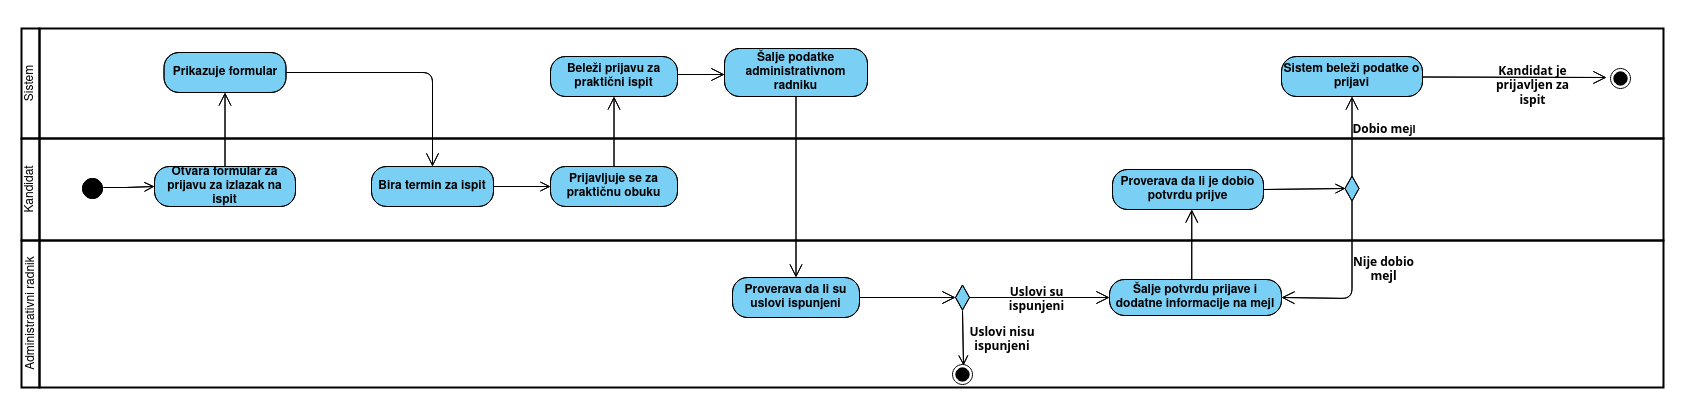
\includegraphics[width=140mm, height=70mm]{Diagrams/dijagram_aktivnosti_prijava_za_praktican_ispit.png}
  \end{center}
  \caption {Dijagram aktivnosti - Prijava za praktični ispit}
  \label{activity_prijava_za_prakticni_ispit}

\end{figure}
